%%%%%%%%%%%%%%%%%%%%%%%%%%%%%%%%%%%%%%%%%%%%%%%%%%%%%%%%%%%%%%%%%%%%%%%%%%%%%%%%
% Лабораторная работа 2 : Измерение модуля Юнга и коэффициента Пуассона
% Выполнили             : Баталов Семен, Хайретдинова Диана, 2021.
%%%%%%%%%%%%%%%%%%%%%%%%%%%%%%%%%%%%%%%%%%%%%%%%%%%%%%%%%%%%%%%%%%%%%%%%%%%%%%%%

\documentclass[12pt, a4paper]{article}
\usepackage[left=2cm, right=2cm, top=2.5cm, bottom=2.5cm, nohead]{geometry}
\usepackage{graphicx}
\usepackage[warn]{mathtext}
\usepackage[utf8]{inputenc}
\usepackage[english, russian]{babel}
\usepackage{indentfirst}
\usepackage{amsmath}
\usepackage{longtable}
\usepackage{multirow}
\usepackage{array}
\usepackage{rotating}
\usepackage{subcaption}
\graphicspath{{pictures/}}

\begin{document}
    
    \newcolumntype{M}[1]{>{\centering\arraybackslash}m{#1}}
    \renewcommand{\arraystretch}{1.2}
    
    \begin{center}
        \large{Санкт-Петербургский Государственный Университет} \\
        \large{Saint-Petersburg State University}\\
        \hfill \break
        \hfill \break
        \hfill \break
        \hfill \break
        \hfill \break
        \hfill \break
        \large{ЛАБОРАТОРИЯ ПРОЧНОСТИ МАТЕРИАЛОВ} \\
        \hfill \break
        \hfill \break
        \hfill \break
        \large{\textbf{ОТЧЕТ}} \\
        \large{\textbf{По лабораторной работе 1}} \\
        \large{<<Измерение модуля Юнга и коэффициента Пуассона>>} \\
        \hfill \break
        \hfill \break
        \hfill \break
        \large{По дисциплине} \\
        \large{<<Лабораторный практикум, лабораторная работа>>} \\
    \end{center}
    
    \hfill \break
    \hfill \break
    \hfill \break
    \hfill \break
    \hfill \break
    \hfill \break
    
    \begin{flushright} 
        \large{Выполнили:} \\
        \hfill \break
        \large{Баталов С. А.} \\
        \large{Хайретдинова Д. Д.} \\
    \end{flushright}
    
    \hfill \break
    \hfill \break
    \hfill \break
    \hfill \break
    \hfill \break
    \hfill \break
    
    \begin{center} 
        \large{Санкт-Петербург} \\
        \large{2021} \\
    \end{center}
    
    \thispagestyle{empty}
    \newpage

\section*{Цель работы}
	Исследование образцов на одноосное
растяжение с измерением деформаций и определением постоянных, характеризующих упругие свойства образца — модуля Юнга Е и коэффициента Пуассона. Знакомство с тензодатчиками сопротивления и их принципом действия. 
\section*{Теоретическое исследование}
	Рассмотрим стержень длины $l = 150 \text{ мм}$, ширины $а = 28.7 мм$ и толщины $b = 2.2 мм$. Площадь сечения  $ S_{0} = 63 мм^{-1}$, стержень растягивается силой Р.
	\begin{figure}[h]
        \centering
        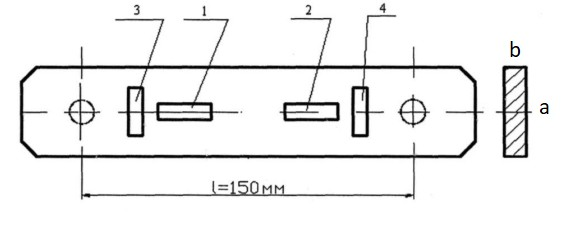
\includegraphics[width = 10cm]{Lab2_1.jpg}
        \caption{Объект испытаний}
        \label{im1}
    \end{figure}
    
     Пусть ось Ох системы координат совпадает с осью стержня. Стержень будет находиться в состоянии одноосного растяжения, то есть напряжения в 
нем равны
\begin{equation}
	\sigma_{xx} = \frac{P}{S_{0}},\quad \sigma_{yy} = \sigma_{zz}			=\sigma_{xy} = \sigma_{xz} = \sigma_{yz} = 0
	\label{eq1}
\end{equation}
Знаем, что поведение материалов при упргой деформации описывается законом Гука, в общем случае закон Гука имеет вид:
\begin{equation}
\begin{aligned}
\varepsilon_{xx} = \frac{1}{E}\Big(\sigma_{xx} - \nu(\sigma_{yy} + \sigma_{zz})\Big); \quad \sigma_{xy} = \frac{E}{1 + \nu}\varepsilon_{xy};
\\
\varepsilon_{yy} = \frac{1}{E}\Big(\sigma_{yy} - \nu(\sigma_{xx} + \sigma_{zz})\Big);\quad  \sigma_{yz} = \frac{E}{1 + \nu}\varepsilon_{yz};
    \\
\varepsilon_{zz} = \frac{1}{E}\Big(\sigma_{zz} - \nu(\sigma_{yy} + \sigma_{xx})\Big); \quad \sigma_{xz} = \frac{E}{1 + \nu}\varepsilon_{xz};
\end{aligned}
\label{eq2}
\end{equation}
Подставив (\ref{eq1}) в (\ref{eq2}), получим, что при данном поле напряжений относительные удлинения по всем осям будут отличны от нуля, а сдвиги будут равны нулю:
\begin{equation}
\varepsilon_{xx} = \frac{1}{E}\sigma_{xx}; \quad \varepsilon_{yy} = \varepsilon_{zz}= - \frac{\nu}{E}\sigma_{xx} \quad \varepsilon_{xy} = \varepsilon_{yz} = \varepsilon_{xz} = 0
\label{eq3}
\end{equation}
Отсюда получим, что экспериментальным путем модуль Юнга и коэффициент Пуассона может быть получен по следующим формулам:
\begin{equation}
E = \frac{P}{S_{0}}\frac{1}{\varepsilon_{xx}}; \quad \nu = - \frac{\varepsilon_{yy}}{\varepsilon_{xx}}
\label{eq4}
\end{equation}
	Относительное удлинение $ \varepsilon_{xx}, \varepsilon_{yy} $ стержня в данной работе находим прямым измерением при помощи тензодатчиков
	
\newpage

\section*{Описание установки}
	В данной лабораторной работе деформации измеряются посредством тензодатчиков, которые установлены в продольном и поперечном направлениях. Тензодатчик (рис.\ref{im2}) состоит из зигзагообразно уложенной проволоки (решетки) $1$, наклеенной на подложку (тонкую бумагу) $2$. К концам проволочной решетки припаяны медные выводы $3$. Сверху решетка покрыта защитным слоем бумаги или лака. Тензодатчик измеряет относительное удлинение в направлении, обозначенном стрелками 

\begin{figure}[h]
        \centering
        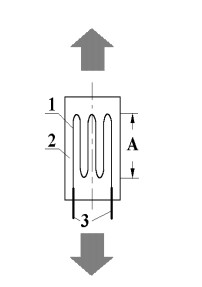
\includegraphics[width = 5cm]{Lab2_2.jpg}
        \caption{Тензодатчик}
        \label{im2}
    \end{figure}

На рисунке \ref{im1} тензодатчики 1 и 2 измеряют продольное удлинение, 3 и 4 поперечное.Тензодатчики подключены к электронному измерителю деформации.Чувствительность датчика характеризуется коэффициентом $K = 6.4 \cdot 10^{-7}$ \\
	Лабораторная работа выполняется на универсальном лабораторном 
стенде посопротивлению материалов(рис \ref{im3}), здесь 1 -- образец, 2 -- нагружающее устройство, 3 -- силоизмерительное устройство
\begin{figure}[h]
        \centering
        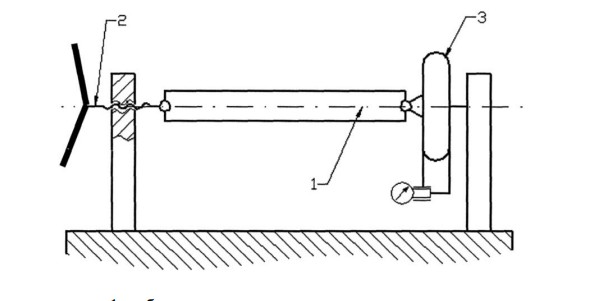
\includegraphics[width = 10cm]{Lab2_3.jpg}
        \caption{Схема экспериментальной установки}
        \label{im3}
    \end{figure}

\newpage
\section*{Экспериментальные данные}
	При выполнении работы расчеты производили, пользуясь пакетом \textbf{Matlab} \\
	Образец нагружали последовательно силой $P$ до $500 Н$ с шагом $ 50Н $ на каждом шагу фиксируя показания измерителя деформаций для 4 тензорезистров. Подсчитали разность показаний измерителя деформаций для ступени $\Delta P = 50 Н$ и занесли в таблицу \ref{tb1}.Усреднили показания и определили приращения деформации$ \varepsilon_{xx}, \varepsilon_{yy}$ , соответствующие приращеню силы по формулам:
	\begin{equation}
	\varepsilon_{xx} = \Delta n_{x} K; \quad \varepsilon_{yy} = \Delta n_{y}K
	\end{equation}

Для каждого шага вычислили постоянные $\nu$ и $ E $.

\begin{table}[h]
\centering
\begin{tabular}{|m{2cm}|m{2.5cm}|m{2.5cm}|m{1.5cm}|m{1.5cm}|m{1.5cm}|m{1.5cm}|m{1.5cm}|}
\hline
Нагрузка P &Продольная  деформация $ \Delta n_{x}$& Поперечная  деформация $\Delta n_{y}$& $\varepsilon_{xx}$ &
$\varepsilon_{yy}$ & $\sigma_{xx}$ & $\nu $& E \\

\hline
Н & Показания ИД, дел. & Показания ИД, дел. & $\cdot 10^{-6} $ & $\cdot 10^{-6} $ &МПа& &ГПа \\
\hline
50&14&-6&8.64&-3.52&0.79&0.43&88.38\\

100&24&-7&15.36&-4.16&1.58&0.29&51.56\\

150&24&-9&15.04&-5.76&2.38&0.37&51.56\\

200&22&-5&13.76&-2.88&3.17&0.23&56.24\\

250&30&-11&19.2&-6.72&3.96&0.37&41.24\\

300 & 27 & -8 & 16.96 & -4.8 & 4.75 & 0.3 & 45.83\\

350&33&-9&20.8&-5.76&5.54&0.27&37.49\\

400&37&-10&23.36&-6.08&6.34&0.27&33.44\\

450&72&-23&46.08&-14.4&7.13&0.32&17.19\\

500 & 55 & -16 & 34.88 &-9.92 &7.92 & 0.29 & 22.5\\
\hline


\end{tabular}
\caption{Экспериментальные и расчетные данные}
\label{tb1}
 \end{table}
 \begin{figure}[h]
        \centering
        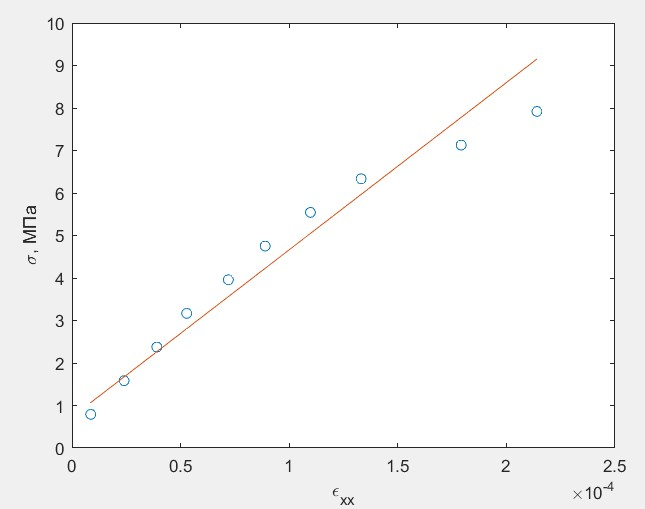
\includegraphics[width = 9cm]{Lab2_4.jpg}
        \caption{График зависимости $\sigma$ от $\varepsilon_{xx}$}
        \label{im2}
    \end{figure}
 Считая, что в 2 последних шагах результаты не являются достоверными, вычислили конечное значение коэффициента Пуассона и модуля Юнга
 \begin{table}[h]
\centering
 \begin{tabular}{|M{2cm}|M{2cm}|M{2cm}|M{2cm}|}
 \hline
 E & $\Delta E$ &  $\nu$ & $\Delta \nu$ \\
 \hline
 ГПа & ГПа &&\\
 \hline
 51 & $\pm$ 12 & 0.32 & $\pm$ 0.01\\
 \hline
 \end{tabular}
 \end{table}
 
 Относительная погрешность измерений
 \begin{equation}
	\frac{E}{\Delta E} = 23\%  \quad \frac{\nu}{\Delta \nu} = 2\%
 \end{equation}
 \\
  \section*{Вывод}
  В проделанной работе исследовали на практике одноосное растяжение стержня, измеряя деформации при помощи тензодачиков, подключенных к измерителю деформаций. Познакомились с принципом работы тезодатчиков сопротивления, их преимуществами и недостатками. Исследовав изменение продольной деформации при увеличении нагрузки убедились в линейной зависимости продольной деформации от напряжения. Вычислили модуль Юнга и коэффициент Пуассона, постоянные, характеризующие упругие свойства материала. Оценили относительные погешности результатов.

\end{document}